\FloatBarrier
\section{Ablation Study}
\label{sec:ablation}

To quantify the contribution of individual pipeline components, two complementary ablation studies were conducted: (A)~a preprocessing pipeline ablation on the deployed SVM model, and (B)~an architecture ablation on the best-performing BiLSTM model. All experiments used the same class-balanced dataset (89,832 samples) and the same stratified 80/20 train--test split with 20\% validation holdout described in Section~\ref{sec:methodology} (seed\,=\,42).

\subsection{Part A --- SVM Preprocessing Ablation}

The SVM baseline (linear kernel, $C = 1$, TF-IDF with 5,000 features) was retrained ten times, each time disabling exactly one of the eight preprocessing steps while keeping all others active.\footnote{The ablation SVM baseline (91.97\%) differs from the main-evaluation SVM (91.80\%, Table~\ref{tab:results}) by 0.17\,pp because the ablation notebook was executed in a separate session on the university-provided Puffer GPU server with a fresh train/validation split, causing minor data-partition variance.} Table~\ref{tab:ablation_configs_a} lists the configurations; Table~\ref{tab:ablation_results_a} reports test-set performance.

\begin{table}[!htb]
\centering
\caption{Part~A configurations --- each row disables one preprocessing step.}
\label{tab:ablation_configs_a}
\footnotesize
\begin{tabular}{@{}cl@{}}
\toprule
\textbf{\#} & \textbf{Configuration} \\
\midrule
0 & Full pipeline (baseline) \\
1 & $-$ Lowercasing \\
2 & $-$ Whitespace stripping \\
3 & $-$ URL removal \\
4 & $-$ Emoji removal \\
5 & $-$ Special character removal \\
6 & $-$ Chat-word expansion \\
7 & $-$ Stopword removal \\
8 & $-$ Lemmatisation \\
9 & No preprocessing (raw text) \\
\bottomrule
\end{tabular}
\end{table}

\begin{table}[!htb]
\centering
\caption[Part~A results]{Part~A results --- SVM test-set performance when each preprocessing step is removed. $\Delta$\,Acc and $\Delta$\,F1 are relative to the full-pipeline baseline.}
\label{tab:ablation_results_a}
\footnotesize
\setlength{\tabcolsep}{3pt}
\begin{tabular}{@{}clcccc@{}}
\toprule
\textbf{\#} & \textbf{Config} & \textbf{Acc\,(\%)} & \textbf{F1\,(\%)} & \textbf{$\Delta$\,Acc} & \textbf{$\Delta$\,F1} \\
\midrule
0 & Full pipeline       & 91.97 & 91.91 & 0.00   & 0.00   \\
1 & $-$ Lowercase       & 91.97 & 91.91 & 0.00   & 0.00   \\
2 & $-$ Whitespace      & 91.97 & 91.91 & 0.00   & 0.00   \\
3 & $-$ URL removal     & 91.95 & 91.89 & $-$0.02 & $-$0.02 \\
4 & $-$ Emoji removal   & 91.97 & 91.91 & 0.00   & 0.00   \\
5 & $-$ Special chars   & 91.97 & 91.91 & 0.00   & 0.00   \\
6 & $-$ Chat-word       & 91.94 & 91.88 & $-$0.03 & $-$0.03 \\
7 & $-$ Stopwords       & 90.64 & 90.56 & $-$1.33 & $-$1.35 \\
8 & $-$ Lemmatisation   & 91.87 & 91.82 & $-$0.10 & $-$0.09 \\
9 & Raw text            & 90.55 & 90.48 & $-$1.42 & $-$1.43 \\
\bottomrule
\end{tabular}
\end{table}

\begin{figure}[!htb]
\centering
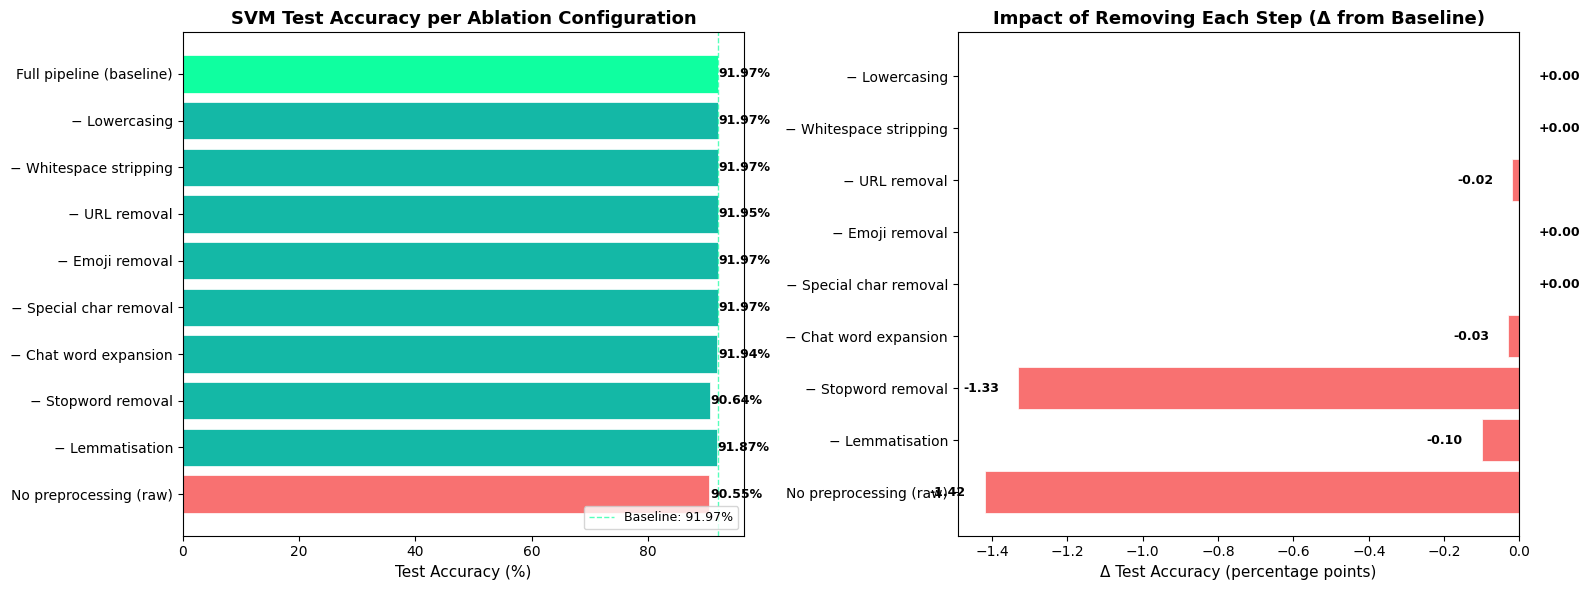
\includegraphics[width=\linewidth]{figures/ablation_study_accuracy.png}
\caption{Part~A: SVM test accuracy per ablation configuration (left) and per-step $\Delta$\,accuracy from the full-pipeline baseline (right).}
\label{fig:ablation_svm}
\end{figure}

Removing \textbf{stopword removal} caused the largest single-step accuracy drop ($-1.33$\,pp), confirming that retaining semantically meaningful function words while removing noise tokens is critical for TF-IDF performance. \textbf{Lemmatisation} was the second most impactful step ($-0.10$\,pp), consolidating morphological variants into shared stems. Four steps (lowercasing, whitespace stripping, emoji removal, special character removal) had zero measurable impact on this corpus, likely because the TF-IDF vocabulary already absorbed their effects. Using raw text without preprocessing reduced accuracy by $1.42$\,pp, underscoring the cumulative value of the full pipeline. Figure~\ref{fig:ablation_svm} visualises the per-step impact; an alternative Accuracy-vs-F1 view is in Appendix Figure~\ref{fig:ablation_svm_f1}.

\FloatBarrier
\subsection{Part B --- BiLSTM Architecture Ablation}

The BiLSTM baseline (2$\times$BiLSTM 256$\rightarrow$128, embedding~dim\,=\,100, dropout\,=\,0.5) was retrained with seven architectural variants spanning depth, capacity, regularisation, and embedding dimensionality.\footnote{The ablation BiLSTM baseline (94.38\%) differs from the main-evaluation BiLSTM (94.70\%, Table~\ref{tab:results}) by 0.32\,pp because the ablation notebook was executed in a separate session on the university-provided Puffer GPU server, causing minor data-partition variance.} Table~\ref{tab:ablation_configs_b} lists the configurations; Table~\ref{tab:ablation_results_b} reports test-set performance.

\begin{table}[!htb]
\centering
\caption{Part~B configurations --- BiLSTM architecture variants.}
\label{tab:ablation_configs_b}
\footnotesize
\begin{tabular}{@{}cl@{}}
\toprule
\textbf{\#} & \textbf{Configuration} \\
\midrule
0 & Baseline (2$\times$BiLSTM 256$\rightarrow$128, emb\,=\,100, drop\,=\,0.5) \\
1 & 1-layer BiLSTM (256 units) \\
2 & 2-layer BiLSTM 128$\rightarrow$64 (smaller) \\
3 & 2-layer BiLSTM 512$\rightarrow$256 (larger) \\
4 & Dropout = 0.3 \\
5 & Dropout = 0.7 \\
6 & Embedding dim = 50 \\
7 & Embedding dim = 200 \\
\bottomrule
\end{tabular}
\end{table}

\begin{table}[!htb]
\centering
\caption{Part~B results --- BiLSTM test-set performance for each architecture variant. $\Delta$\,Acc and $\Delta$\,F1 are relative to the baseline.}
\label{tab:ablation_results_b}
\footnotesize
\setlength{\tabcolsep}{3pt}
\begin{tabular}{@{}clcccc@{}}
\toprule
\textbf{\#} & \textbf{Config} & \textbf{Acc\,(\%)} & \textbf{F1\,(\%)} & \textbf{$\Delta$\,Acc} & \textbf{$\Delta$\,F1} \\
\midrule
0 & Baseline            & 94.38 & 94.33 & 0.00   & 0.00   \\
1 & 1-layer (256)       & 93.16 & 93.13 & $-$1.22 & $-$1.20 \\
2 & 128$\rightarrow$64  & 94.06 & 94.03 & $-$0.32 & $-$0.30 \\
3 & 512$\rightarrow$256 & 94.67 & 94.65 & $+$0.29 & $+$0.32 \\
4 & Dropout 0.3         & 94.03 & 94.01 & $-$0.35 & $-$0.32 \\
5 & Dropout 0.7         & 93.89 & 93.83 & $-$0.49 & $-$0.50 \\
6 & Emb dim 50          & 93.84 & 93.83 & $-$0.54 & $-$0.50 \\
7 & Emb dim 200         & 94.47 & 94.45 & $+$0.09 & $+$0.12 \\
\bottomrule
\end{tabular}
\end{table}

Reducing depth to a single layer (\#1) caused the largest accuracy drop ($-1.22$\,pp), confirming that the second BiLSTM layer captures additional contextual dependencies essential for emotion discrimination. Increasing capacity to 512$\rightarrow$256 (\#3) yielded a modest gain ($+0.29$\,pp) at the cost of 51\% more parameters (11.2\,M vs.\ 7.4\,M), suggesting diminishing returns beyond the baseline capacity. Dropout of 0.7 (\#5) degraded performance by $0.49$\,pp, indicating over-regularisation, while dropout of 0.3 (\#4) also reduced accuracy ($-0.35$\,pp), confirming that 0.5 is near-optimal. Halving the embedding dimension (\#6) reduced accuracy by $0.54$\,pp; doubling it to 200 (\#7) provided only a marginal $+0.09$\,pp gain, confirming that 100-dimensional embeddings are sufficient for this vocabulary size. Figure~\ref{fig:ablation_bilstm} visualises the per-variant impact; an alternative Accuracy-vs-F1 view is in Appendix Figure~\ref{fig:ablation_bilstm_f1}.

\begin{figure}[!htb]
\centering
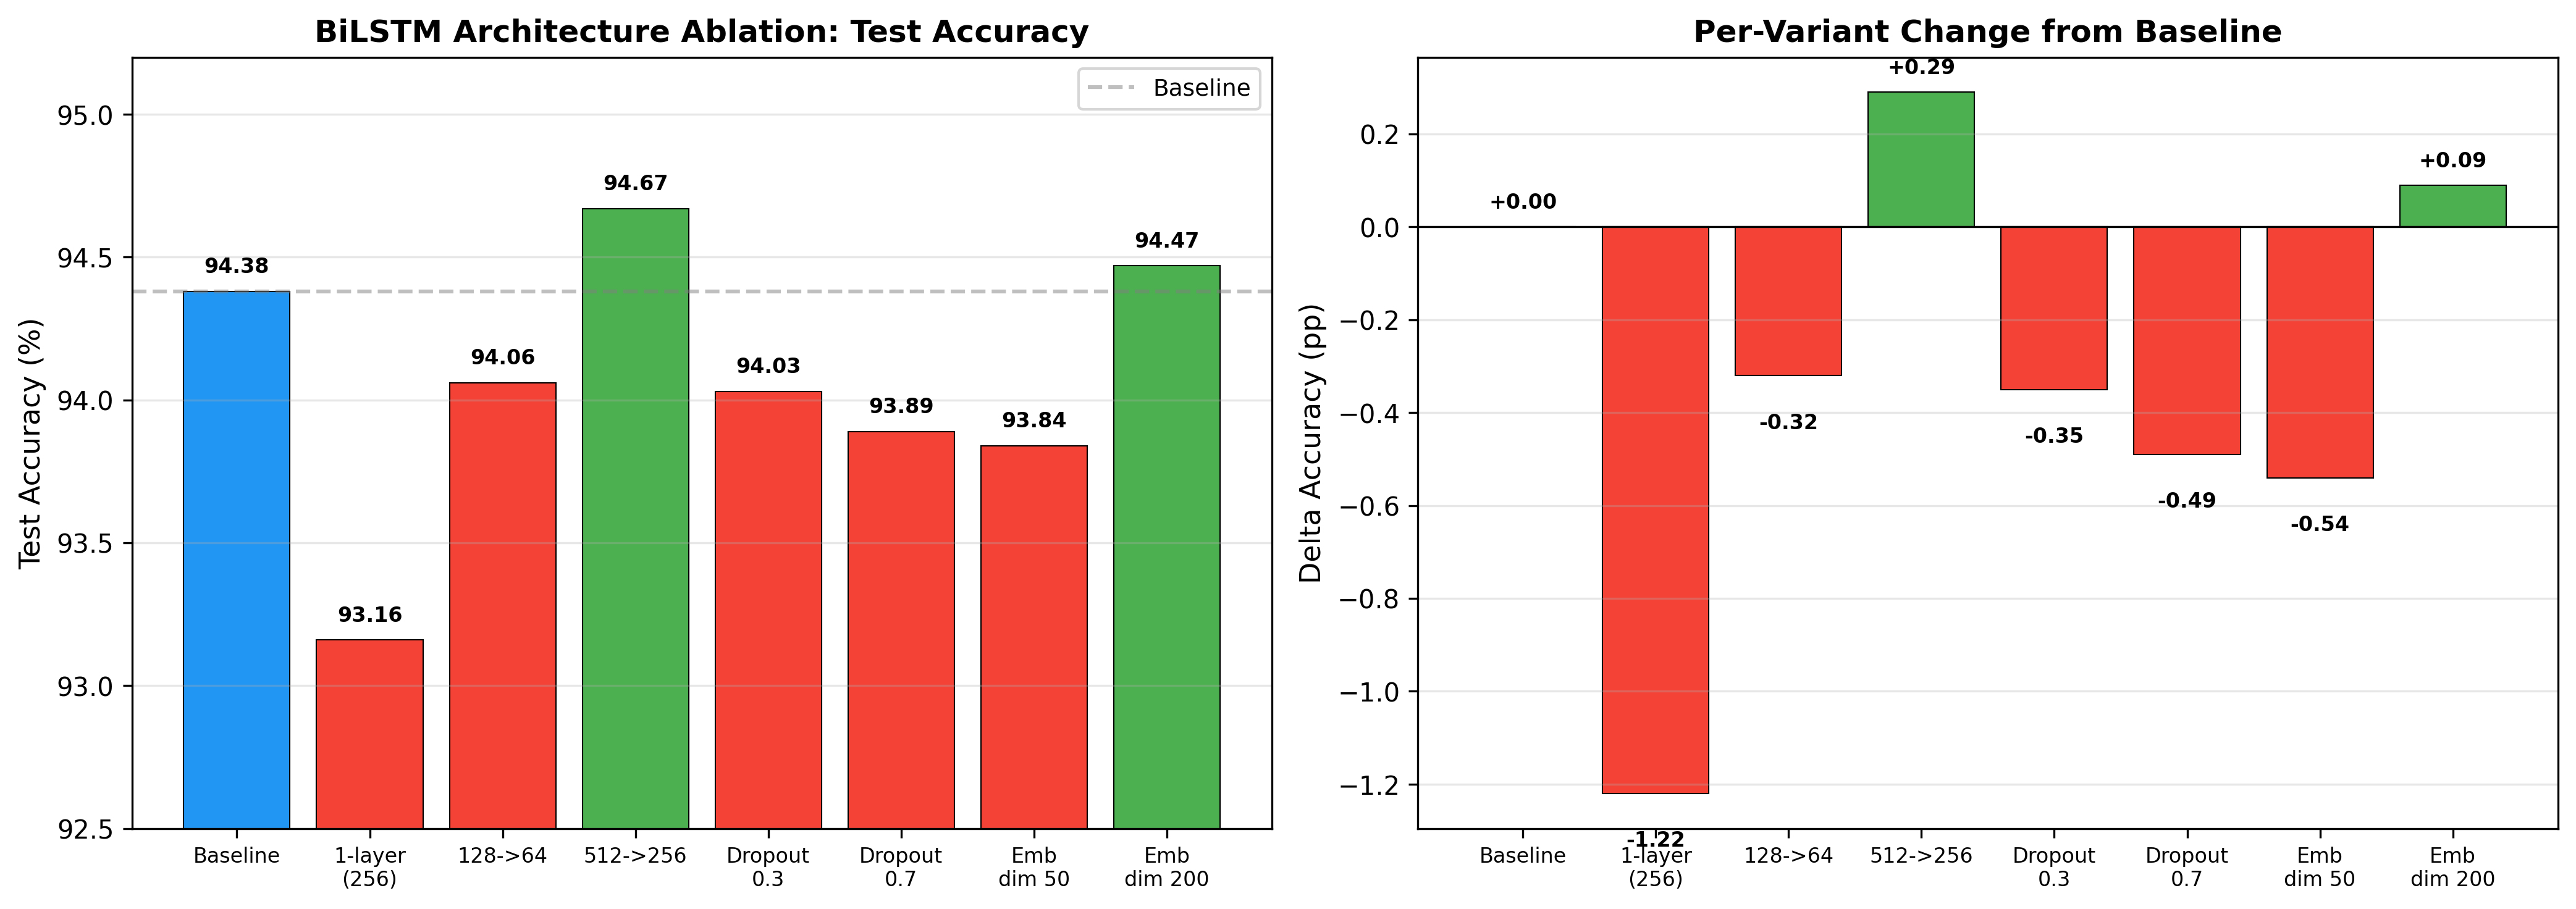
\includegraphics[width=\linewidth]{figures/ablation_bilstm_architecture.png}
\caption{Part~B: BiLSTM test accuracy per architecture variant (left) and per-variant $\Delta$\,accuracy from the baseline (right).}
\label{fig:ablation_bilstm}
\end{figure}

\subsection{Ablation Summary}

The preprocessing ablation demonstrates that text normalisation is not optional: the full eight-step pipeline contributes $1.42$\,pp over raw text for SVM, with stopword removal alone accounting for $1.33$\,pp. The architecture ablation indicates that the 2$\times$BiLSTM 256$\rightarrow$128 configuration is near-optimal, with depth ($-1.22$\,pp for single-layer) and embedding dimensionality ($-0.54$\,pp for dim\,=\,50) being the most sensitive hyperparameters.
